\documentclass[]{report}
\usepackage{kotex}
\usepackage{verbatim} 
\usepackage{graphicx} 

\usepackage{listings}
\usepackage{color}

\definecolor{dkgreen}{rgb}{0,0.6,0}
\definecolor{gray}{rgb}{0.5,0.5,0.5}
\definecolor{mauve}{rgb}{0.58,0,0.82}

\lstset{frame=tb,
	language=Python,
	aboveskip=3mm,
	belowskip=3mm,
	showstringspaces=false,
	columns=flexible,
	basicstyle={\small\ttfamily},
	numbers=none,
	numberstyle=\tiny\color{gray},
	keywordstyle=\color{blue},
	commentstyle=\color{dkgreen},
	stringstyle=\color{mauve},
	breaklines=true,
	breakatwhitespace=true,
	tabsize=3
}


% Title Page
\title{HW07 - REPORT}
\author{정보컴퓨터공학부 201624536 이국현}


\begin{document}
\maketitle


\chapter{서론}

\section{Linear SVM Classifiers}

\begin{figure}[ht!]
    \centering
    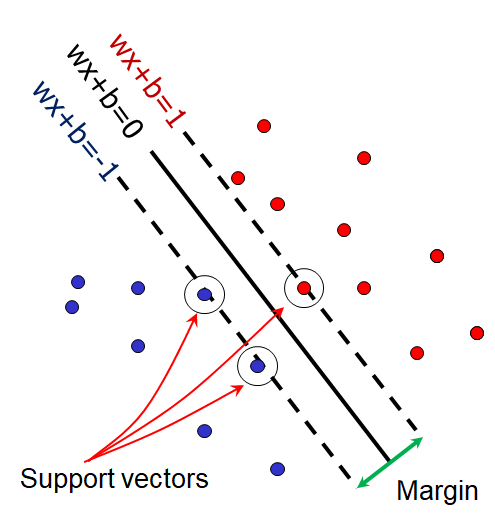
\includegraphics[width=0.5\textwidth]{image/SVM.png}
    \caption{Linear SVM Classifiers}
    \label{SVM}
\end{figure}

x, y 좌표와 해당하는 class가 주어진 Training data가 있다면
Machine learning을 통해 class를 구분 짓는 기준을 정할 수 있다.
이 기준을 좌표 상의 Line으로 그릴 수 있다면 이 Model을 Linear classifier라고 한다. 
대표적으로 Support vector machine이 있다. 두 그룹 사이에 수없이 많은 선을 그릴 수 있지만,
SVM에서는 \ref{SVM}과 같이 두 그룹까지의 Margin을 최대화하는 Line을 Model로 학습한다.  \\

\section{Non-linear SVM Classifiers}

\begin{figure}[ht!]
    \centering
    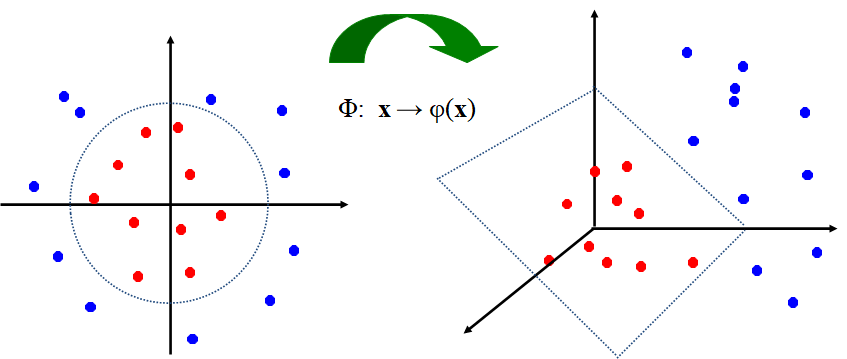
\includegraphics[width=1\textwidth]{image/pi.png}
    \caption{Non-linear SVM Classifiers}
    \label{pi}
\end{figure}

\ref{SVM}의 왼쪽 그림과 같이 두 그룹의 경계가 선형적이지 않은 경우 이를 Non-linear classifier라고 한다. 
이 경우에는 SVM으로 Model을 생성할 수 없다. 하지만 좌표를 3차원으로 확장할 수 있다면, 
그 함수에 따라서 \ref{SVM}과 같이 두 그룹을 구분하는 Plane을 생성할 수도 있다.  \\

\[ K(x_i, x_j) = \exp(-\frac{||x_i - x_j||^2}{2\sigma^2})\]

2D 좌표를 3차원으로 확장하는 여러 가지 함수가 있지만, 일반적으로 많이 사용되는 Gaussian RBF 함수를 사용할 것이다. \\


\chapter{본론}

\section{Linear SVM Classifiers}

\begin{lstlisting}
l_pRandomState = [20, 30, 40]
l_pC1 = [10, 1, 0.1]

def prob1():
	for row, pRandomState in enumerate(l_pRandomState):
		# data 생성
		coords, labels = datasets.make_blobs(
			n_samples=100, cluster_std=1.2, random_state=pRandomState, centers=2)

		plt.figure(figsize=(16, 5))
		for col, pC in enumerate(l_pC1):
			plt.subplot(1, 3, col + 1)
			ax = plt.gca()
			ax.set_title('C=a%.1f' % pC)

			# liner kernel을 이용해 SVM classifier 생성
			clf = SVC(kernel="linear", C=pC)
			clf.fit(coords, labels)

			# SVM classifier model을 통해 line 그래프 생성
			inspection.DecisionBoundaryDisplay.from_estimator(
				clf,
				coords,
				plot_method="contour",
				levels=[-1, 0, 1],
				linestyles=["--", "-", "--"],
				ax=ax,
			)

			# label에 따라 분리하여 scatter 그래프 생성
			plt.scatter(coords[labels == 0, 0], coords[labels == 0, 1])
			plt.scatter(coords[labels == 1, 0], coords[labels == 1, 1])
			plt.scatter(clf.support_vectors_[:, 0], clf.support_vectors_[
				:, 1], s=250, alpha=0.3)
		plt.show()	
\end{lstlisting}

sklearn의 datasets.make\_blobs을 사용하여 Training data를 생성하였다. 
생성된 Training data를 통해 SVM model을 생성하고 그래프에 Line과 Support vectors를 표시해 주었다. 


\section{Non-linear SVM Classifiers}

\subsection{Create Data}

\begin{lstlisting}
def createDatasets():
	# data 생성
	coords, labels = datasets.make_circles(
		n_samples=100, factor=0.1, noise=0.1)

	# label에 따라 분리하여 scatter 그래프 생성
	plt.scatter(coords[labels == 0, 0], coords[labels == 0, 1])
	plt.scatter(coords[labels == 1, 0], coords[labels == 1, 1])
	plt.show()
	return [coords, labels]
\end{lstlisting}

sklearn의 datasets.make\_circles을 사용하여 Training data를 생성하였다. 


\subsection{Kernel function}

\begin{lstlisting}
def gauss_rbf(coords):
	# 2차원 coordinates를 gaussian rbf를 통해 3차원으로 확장
	X = coords[:, 0]
	Y = coords[:, 1]
	Z = np.exp(-(X**2 + Y**2))
	return X, Y, Z

def kernelFunction(coords, labels):
	fig = plt.figure()
	ax = fig.add_subplot(projection='3d')
	X, Y, Z = gauss_rbf(coords)

	# label에 따라 분리하여 scatter 그래프 생성
	ax.scatter(X[labels == 0], Y[labels == 0], Z[labels == 0])
	ax.scatter(X[labels == 1], Y[labels == 1], Z[labels == 1])
	plt.show()
\end{lstlisting}

make\_circles로 생성된 Training data는 Linear classifier로 class를 구분할 수 없기 때문에,
Gaussian RBF 함수를 Kernel function으로 설정하여 3차원으로 확장하였다. 
이때 기준이 되는 X는 원점(0, 0)이기 때문에 생략하였다.  \\



\subsection{Train SVM}

\begin{lstlisting}

def trainSVM(coords, labels):
	plt.figure(figsize=(10, 5))
	for col, pC in enumerate(l_pC2):
		plt.subplot(1, 2, col + 1)
		ax = plt.gca()
		ax.set_title('C=%.1f' % pC)

		# rbf kernel을 이용해 SVM classifier 생성
		clf = SVC(kernel="rbf", C=10)
		clf.fit(coords, labels)

		# SVM classifier model을 통해 line 그래프 생성
		inspection.DecisionBoundaryDisplay.from_estimator(
			clf,
			coords,
			plot_method="contour",
			levels=[-1, 0, 1],
			linestyles=["--", "-", "--"],
			ax=ax,
		)

		# label에 따라 분리하여 scatter 그래프 생성
		plt.scatter(coords[labels == 0, 0], coords[labels == 0, 1])
		plt.scatter(coords[labels == 1, 0], coords[labels == 1, 1])
	plt.show()

\end{lstlisting}

make\_circles로 생성된 Training data는 Linear classifier로 class를 구분할 수 없기 때문에, 
Gaussian RBF 함수를 Kernel function으로 설정하여 SVM을 학습하였다.  
학습한 Non-linear SVM classifier model을 그래프에 표시해 주었다. \\


\chapter{결론}

\section{Linear SVM Classifiers}

\begin{figure}[ht!]
    \centering
    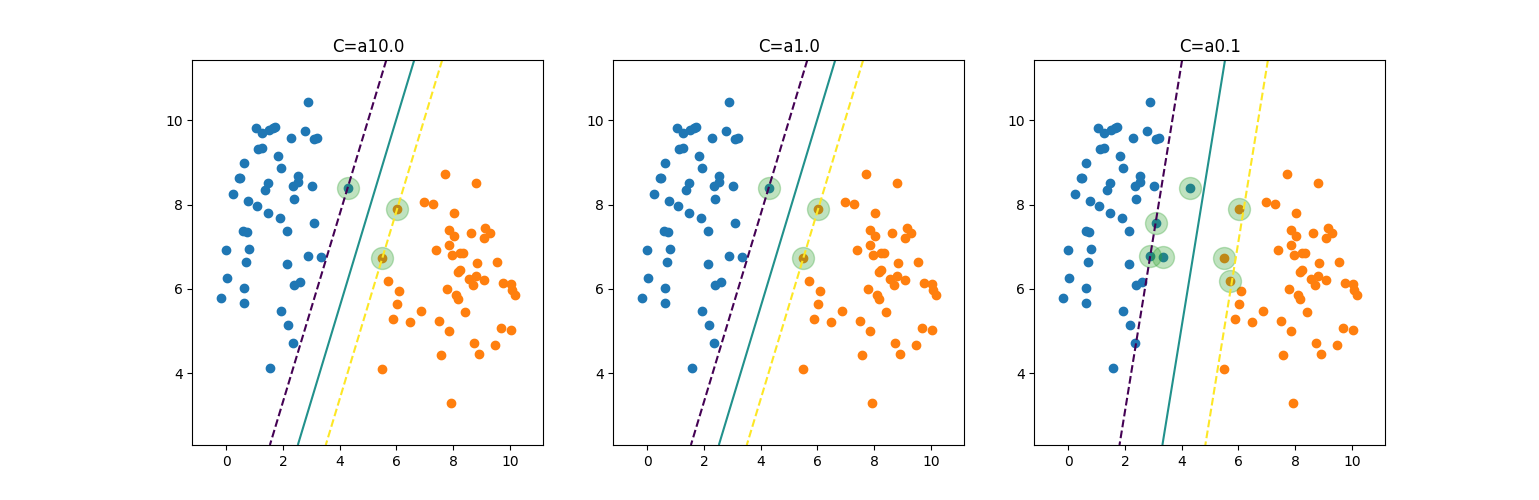
\includegraphics[width=1\textwidth]{image/1-1.png}
    \caption{random\_state=20}
    \label{1-1}
\end{figure}

\begin{figure}[ht!]
    \centering
    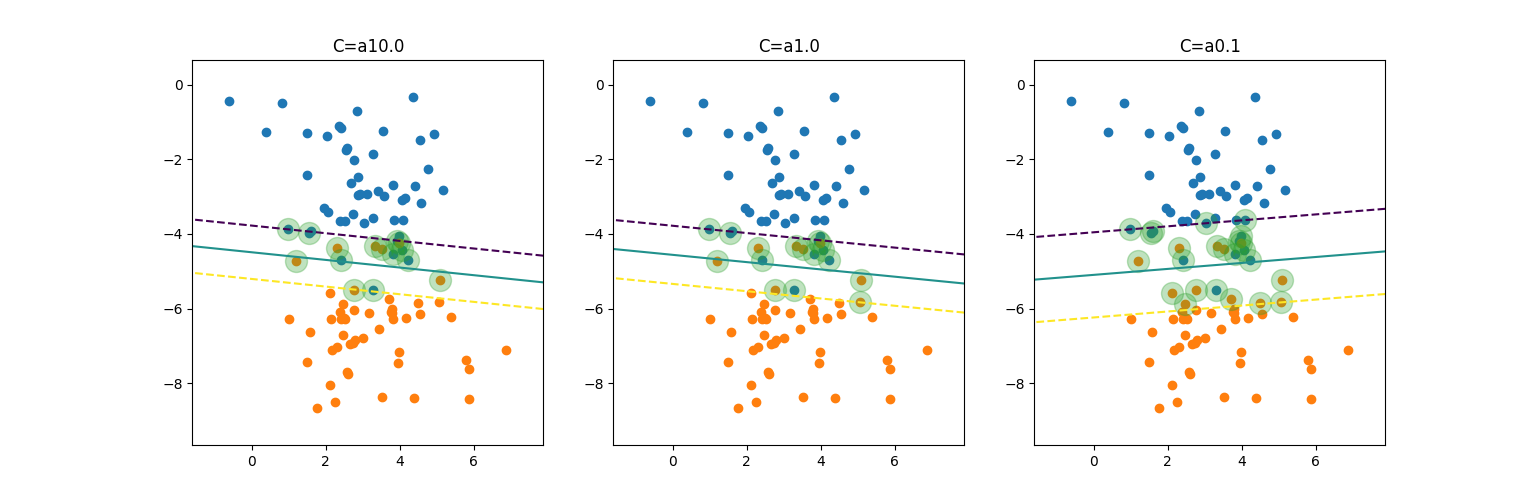
\includegraphics[width=1\textwidth]{image/1-2.png}
    \caption{random\_state=30}
    \label{1-2}
\end{figure}

\begin{figure}[ht!]
    \centering
    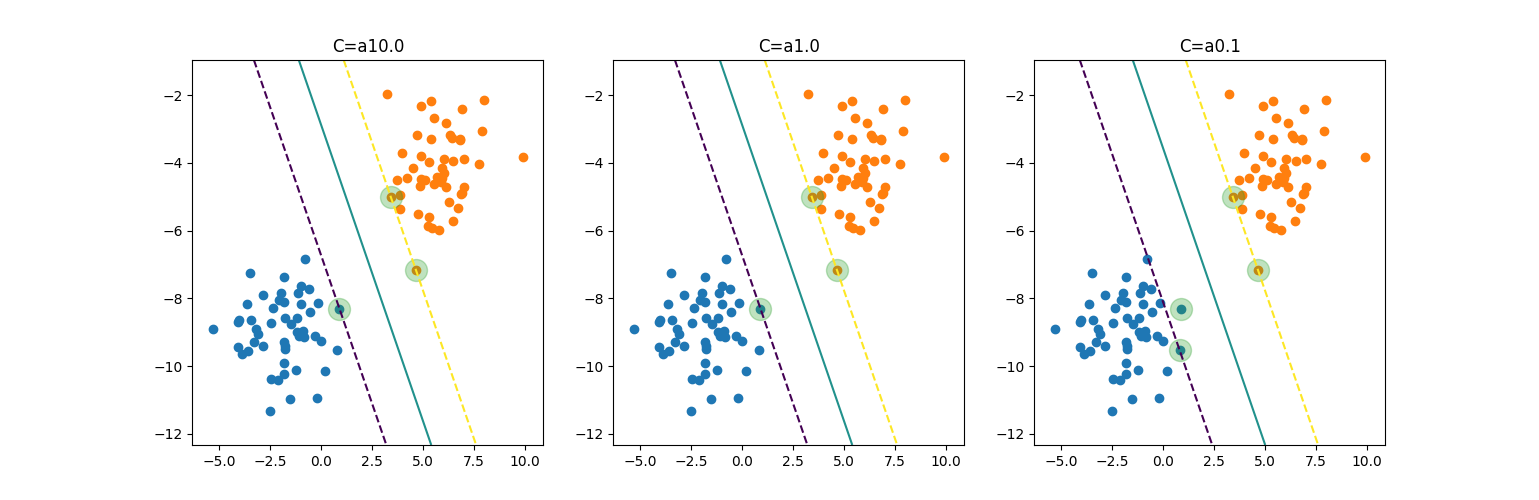
\includegraphics[width=1\textwidth]{image/1-3.png}
    \caption{random\_state=40}
    \label{1-3}
\end{figure}

생성한 데이터 별로 Support vector machine을 적용하여 Model을 생성하였다. 
C(Misclassifications cost) 값을 크게 설정할수록 Suuport vector가 많아지는 것을 확인할 수 있다.  \\


\section{Non-linear SVM Classifiers}

\subsection{Create Data}

\begin{figure}[ht!]
    \centering
    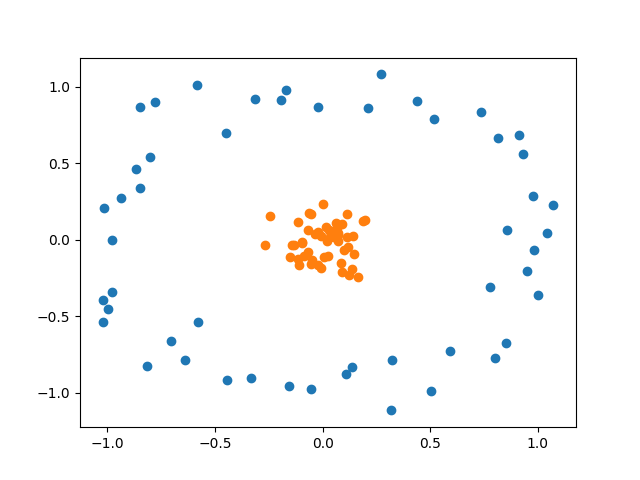
\includegraphics[width=0.5\textwidth]{image/2-1.png}
    \caption{Circle data}
    \label{2-1}
\end{figure}

make\_circles로 생성된 Data는 class 0 (파란색)은 바깥쪽에 원형 고리 형태를 형성하고,
class 1 (주황색)은 중심에 모인 형태를 형성하여 Linear classifier로는 구분할 수 없다.  \\


\subsection{Kernel function}

\begin{figure}[ht!]
    \centering
    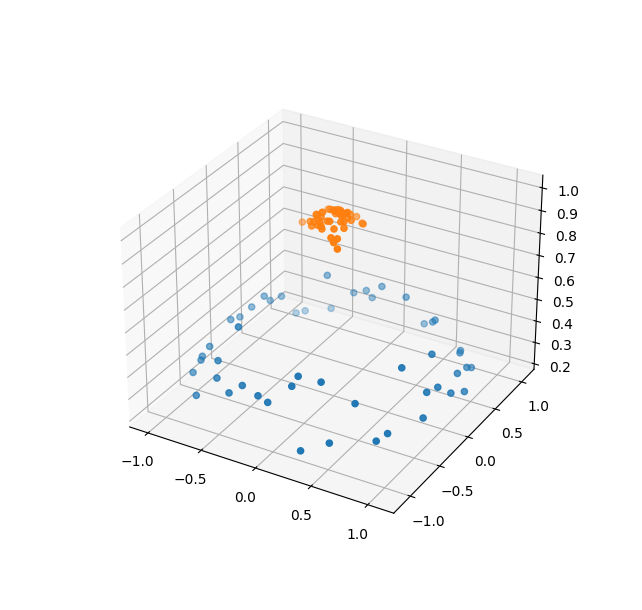
\includegraphics[width=0.7\textwidth]{image/2-2.png}
    \caption{Gaussian RBF}
    \label{2-2}
\end{figure}

Circle data에 Gaussian RBF 함수를 이용해 3차원으로 확장한 결과
plane으로 구분할 수 있는 Figure \ref{2-2}의 형태를 형성하였다. \\

\subsection{Train SVM}

\begin{figure}[ht!]
    \centering
    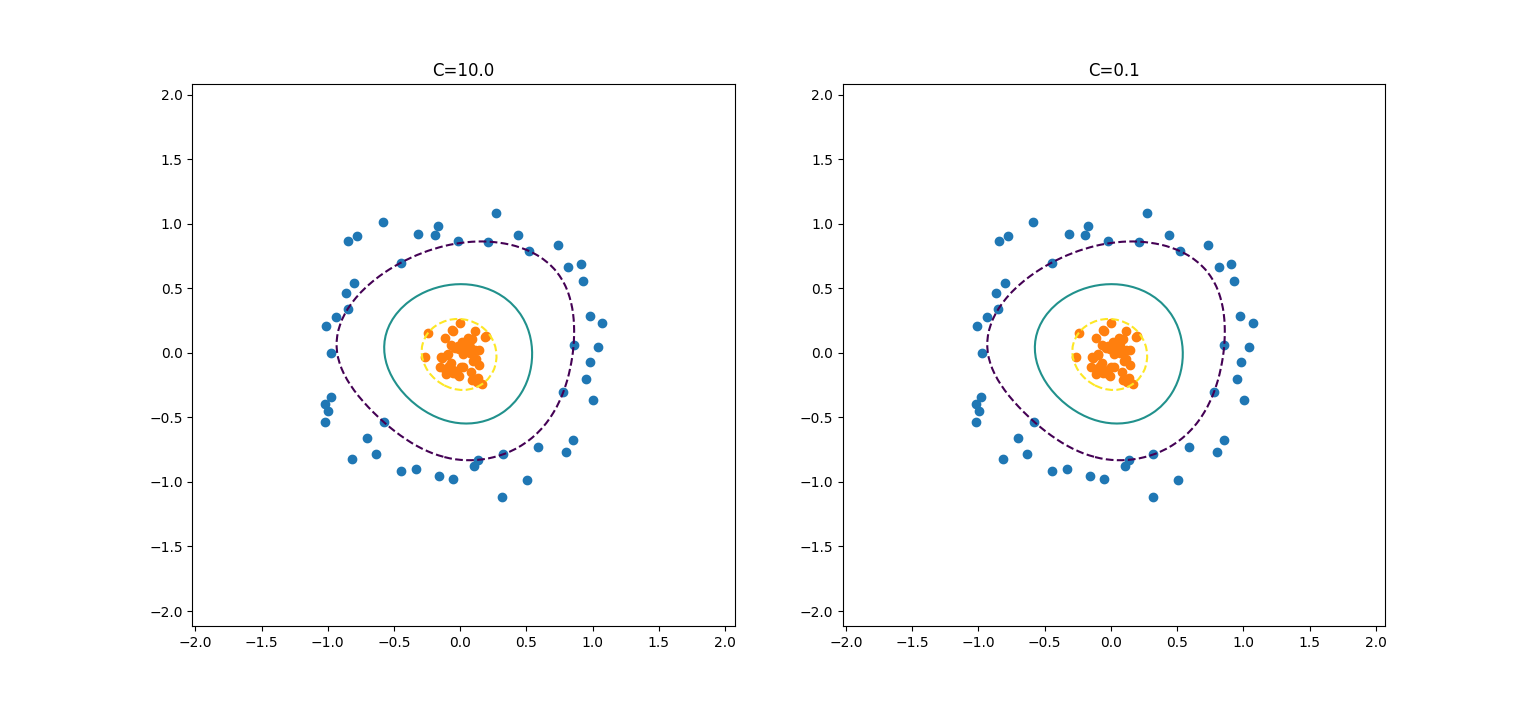
\includegraphics[width=1.0\textwidth]{image/2-3.png}
    \caption{factor=0.1}
    \label{2-3}
\end{figure}

Gaussian RBF 함수를 Kernel funciton으로 이용해 SVM을 통해
Non-linear classifier model을 생성할 수 있었다.  \\

\end{document}          

